\section{Introduction to the New Model}
This chapter introduces a new ``top-down'' Continuous and Proactive Security Assessment Model (CAPSAM) framework as a response to limitations in traditional risk assessment approaches. The case study by \citet{shaikh2023information} addressed the reactive nature of the Top Management Team (TMT)'s attention in its influence on the decision to carry out an Information Security Risk Assessment (ISRA). This reinforces the need for a new proactive, continuous security model that integrates information security across all layers of an organisation.

\section{Overview of the CAPSAM Framework}
    \subsection{Purpose, Goals, and Intended Outcomes}
    The CAPSAM framework is designed to \textbf{address the limitations of cybersecurity models} by emphasising a proactive and continuous approach to risk assessment. Its primary purpose is to \textbf{integrate information security considerations from the earliest stages of system development} and throughout its lifecycle.

    The main goal of CAPSAM is to minimise the likelihood and impact of cybersecurity breaches through vigilant, ongoing risk management. The model aims to \textbf{integrate information security across all layers of an organisation} and focuses on continuous improvement, ensuring a resilient security posture that adapts to the ever-changing threat landscape. By doing this, CAPSAM prioritises the protection of all stakeholders\textemdash including the customer and their data\textemdash strengthening overall organisational security and trust.

    \subsection{The Five Pillars of CAPSAM}
    The core philosophies of CAPSAM can be summarised in five pillars: \textbf{Culture, Continuous, Auditing, Response, Proactive (CCARP)}. These pillars are illustrated in Figure \ref{fig:CAPSAM} and form the foundation of the model's approach to information security risk management.

    \begin{figure}[htbp]
        \centering
        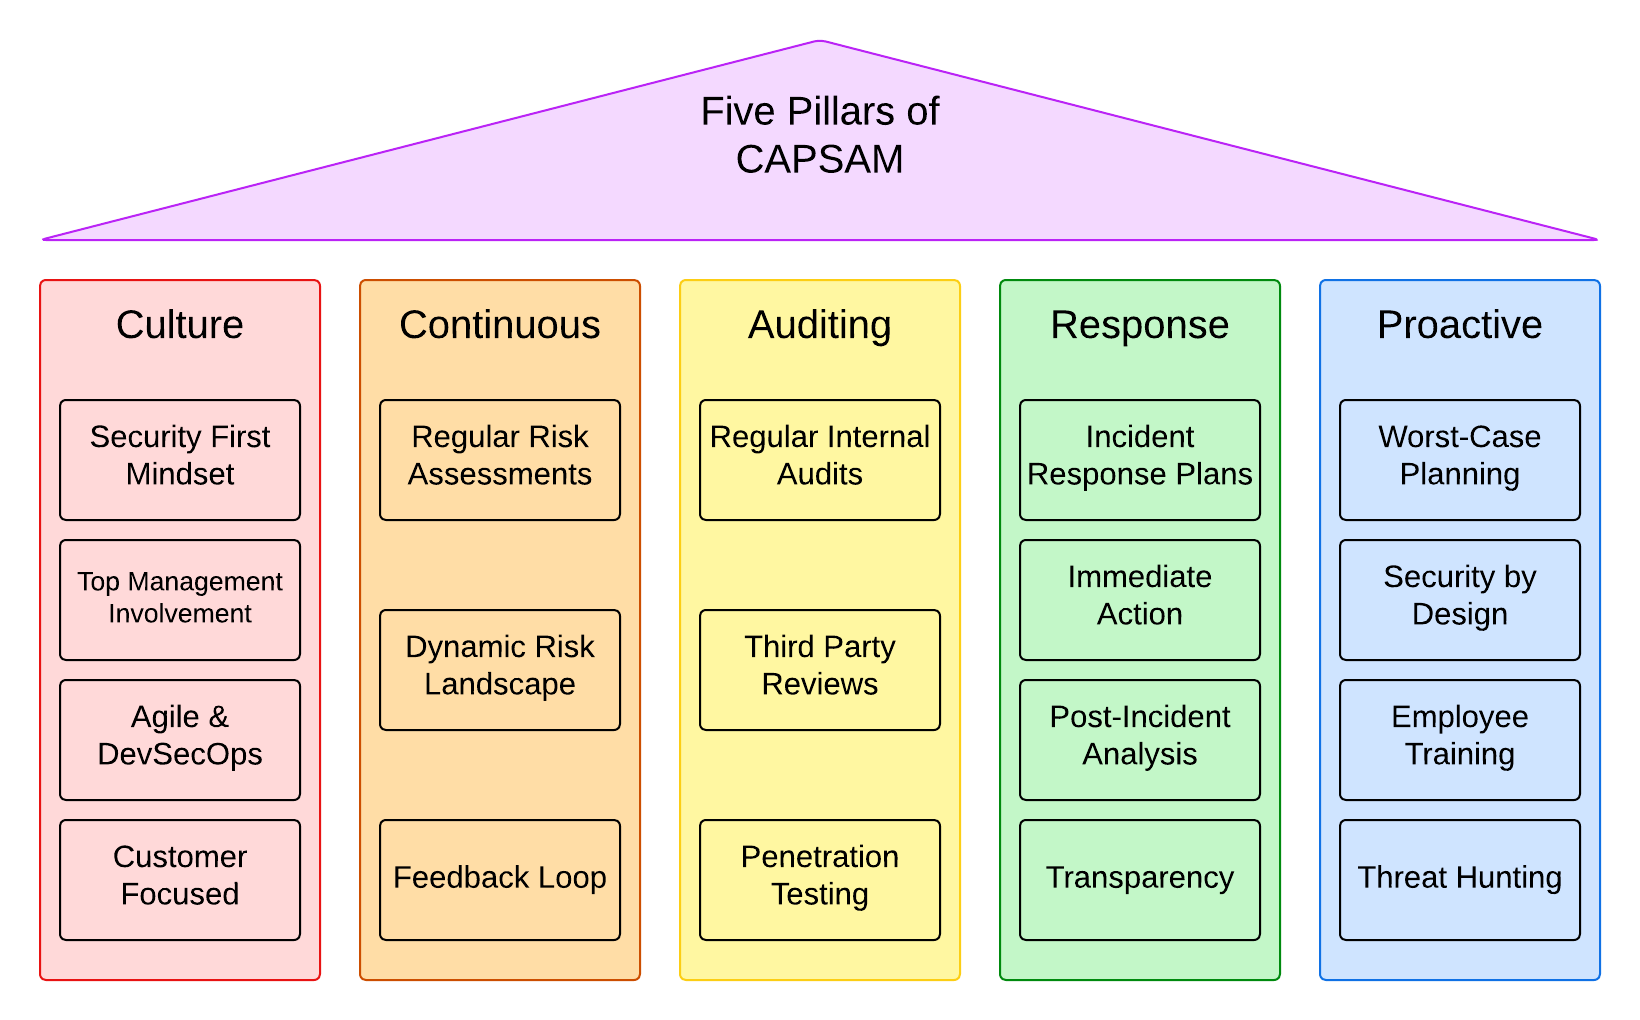
\includegraphics[width=0.8\textwidth]{figures/CAPSAM-Pillars.png}
        \caption{The Five Pillars of CAPSAM: Culture, Continuous, Auditing, Response, and Proactive (CCARP) and their components.}
        \label{fig:CAPSAM}
    \end{figure}

    \begin{itemize}
        \item \textbf{Culture:}
        \begin{itemize}
            \item \textbf{Security First Mindset:}
            \item \textbf{Top Management Involvement:}
            \item \textbf{Agile \& DevSecOps:}
            \item \textbf{Customer Focused:}
        \end{itemize}
        \item \textbf{Continuous:}
        \begin{itemize}
            \item \textbf{Regular Risk Assessments:}
            \item \textbf{Dynamic Risk Landscape:}
            \item \textbf{Feedback Loop:}
        \end{itemize}
        \item \textbf{Auditing:}
        \begin{itemize}
            \item \textbf{Regular Internal Audits:}
            \item \textbf{Third Party Reviews:}
            \item \textbf{Penetration Testing:}
        \end{itemize}
        \item \textbf{Response:}
        \begin{itemize}
            \item \textbf{Incident Response Plans:}
            \item \textbf{Immediate Action:}
            \item \textbf{Post-Incident Analysis:}
            \item \textbf{Transparency:}
        \end{itemize}
        \item \textbf{Proactive:}
        \begin{itemize}
            \item \textbf{Worst-Case Planning:}
            \item \textbf{Security by Design:}
            \item \textbf{Employee Training:}
            \item \textbf{Threat Hunting:}
        \end{itemize}
    \end{itemize}

    \subsection{FAMRM Cycle}
    The CAPSAM framework operates within the FAMRM cycle (New \textbf{Feature}, Information Security Risk \textbf{Assessment}, Proactive \textbf{Mitigation} Strategies, Incident \textbf{Response} Planning, and Continuous Threat \textbf{Monitoring}). This cycle ensures that each new feature or system development is subject to proactive mitigation strategies, and continuous risk assessments where feedback loops inform the next ISRA. The FAMRM cycle is illustrated in Figure \ref{fig:FAMRM}.

    \begin{figure}[htbp]
        \centering
        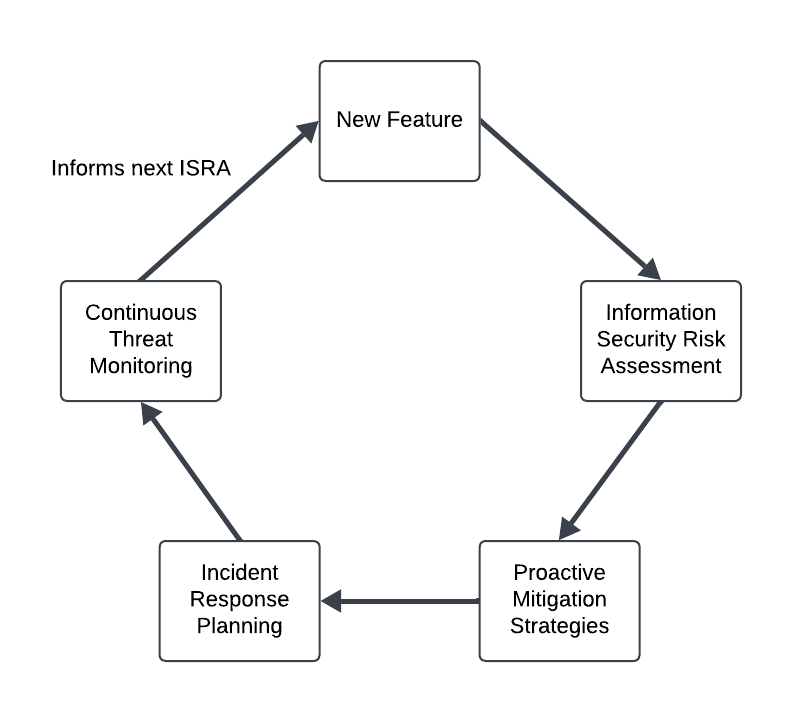
\includegraphics[width=0.6\textwidth]{figures/FAMRM-Cycle.png}
        \caption{FAMRM Cycle for Integrating Security into New Feature Development, Highlighting Continuous Risk Assessment, Proactive Mitigation, and Feedback Loops in Agile and DevSecOps Environments.}
        \label{fig:FAMRM}
    \end{figure}

\section{Justification for a Top-Down Approach}
    \subsection{Importance of Top-Down Risk Management}
    Explain the necessity of a top-down approach in information security risk management. Contrast this with the limitations of a bottom-up approach, which may be more reactive. Emphasize the need for executive engagement in setting priorities, allocating resources, and enforcing security policies.

    \subsection{Alignment with Corporate Governance}
    Discuss how a top-down approach aligns with corporate governance and strategic business objectives. Outline the benefits of ensuring top-level involvement in risk management processes.

    \subsection{Limitations of Bottom-Up Approaches}
    Describe the challenges of relying on bottom-up approaches, such as lack of management buy-in and difficulty in achieving holistic, coordinated efforts across departments.

\section{Theoretical Foundations}
    \subsection{Attention-Based View (ABV) and Proactive Security}
    Introduce the Attention-Based View theory, explaining its core concepts related to limited attention capacity for non-routine activities. Discuss how CAPSAM applies ABV to ensure information security is continuous and proactive.

    \subsection{Agile Methodology and DevSecOps Principles}
    Describe how agile methodologies and DevSecOps principles support continuous integration, delivery, and security practices. Relate this to CAPSAM’s focus on continuous feedback and improvement loops.

    \subsection{ISO 31000: Risk Management Standard}
    Discuss ISO 31000 and its relevance to CAPSAM. Emphasize how the risk management structure of ISO 31000 informs CAPSAM’s approach to risk analysis, evaluation, and treatment.

    \subsection{Organisational Learning and Continuous Feedback}
    Highlight the importance of continuous learning and feedback loops in CAPSAM. Connect this to principles of organisational learning and explain how feedback drives improvement in security measures.

    \subsection{Customer-Focused Approach and Trust Theory}
    Discuss how a customer-focused approach enhances trust and aligns with corporate social responsibility principles. Introduce trust theory and explain how it is integrated into CAPSAM to improve stakeholder engagement and organisational security.

\section{Critical Analysis and Justification}
    \subsection{Strengths of CAPSAM}
    Critically analyse the strengths of the CAPSAM model, such as its proactive nature, emphasis on stakeholder engagement, and its continuous improvement cycle. Use sources to support your claims on the benefits of proactive risk management.

    \subsection{Limitations of CAPSAM}
    Acknowledge the limitations and challenges of implementing CAPSAM. Discuss aspects such as the need for continuous updates to risk assessments, the resources required for ongoing monitoring, and the potential for over-reliance on specific teams or individuals.

    \subsection{Comparison with Case Study Approach}
    Compare CAPSAM with the reactive approach in the case study. Highlight how CAPSAM’s proactive, top-down, and continuous nature addresses the gaps and limitations of the case study approach.

    \subsection{Challenges in Implementing CAPSAM}
    Discuss potential challenges in implementing CAPSAM, such as obtaining management support, ensuring consistent communication across departments, and managing the resources needed for continuous monitoring.

\section{Implementation of CAPSAM}
    \subsection{Phase 1: Planning and Preparation}
    Outline the first phase of implementing CAPSAM, which involves identifying key stakeholders, defining roles and responsibilities, and establishing communication channels. Discuss the importance of aligning the security risk management policy with the organisation’s overall strategy.

    \subsection{Phase 2: Implementation}
    Describe the process of conducting risk assessments, identifying vulnerabilities, prioritizing risks, and developing mitigation strategies. Explain the importance of integrating risk management activities with the software development lifecycle.

    \subsection{Phase 3: Review and Improvement}
    Detail the review phase, which involves regular assessments of the CAPSAM framework, adapting the model based on insights and business changes, and fostering a culture of continuous security improvement.

\section{Conclusion}
Summarize the key points discussed in the chapter, reinforcing the value of the CAPSAM framework in overcoming the limitations of traditional risk assessment models. Emphasize the importance of a proactive, continuous approach to information security and its alignment with business practices and strategic goals.